\documentclass[conference,leqno]{IEEEtran}
\IEEEoverridecommandlockouts
% Template version as of 6/27/2024

\usepackage{cite}
\usepackage{amsmath,amssymb,amsfonts}
\usepackage{algorithmic}
\usepackage{graphicx}
\usepackage{textcomp}
\usepackage{xcolor}
\usepackage[section]{placeins}

\def\BibTeX{{\rm B\kern-.05em{\sc i\kern-.025em b}\kern-.08em
T\kern-.1667em\lower.7ex\hbox{E}\kern-.125emX}}

\begin{document}

\title{Final Project: Few-Shot Detection of Bioacoustic Events}

\author{
\IEEEauthorblockN{Vicente Jos\'e Escarigo Miranda}
\IEEEauthorblockA{
\textit{UAM, Universidad Autonoma de Madrid} \\
\\
} }

\maketitle

\begin{abstract}
This report presents a lightweight few-shot bioacoustic event detection system
for DCASE 2023 Task 5. I start from the official prototypical-network baseline
and focus on feasible, evaluation-aware improvements without external data or
heavy backbones. Audio is converted to PCEN features with delta-MFCCs, encoded
by a shallow ResNet, and classified by distances to positive and negative
prototypes. I use adaptive segmentation at evaluation, negative sampling from
gaps between supports, optional transductive refinement of prototypes, and
simple duration-based post-processing. On the validation set, the proposed
configuration achieves 39.02\% F1 (precision 45.67\%, recall 34.06\%), improving
the official prototypical baseline by 9.43 absolute F1. The study highlights
which components most affect performance under the task’s strict 5-shot
protocol and provides a reproducible reference for further experimentation.
\end{abstract}

\begin{IEEEkeywords}
few-shot learning, bioacoustics, sound event detection, embeddings, prototypical
methods, event-based evaluation
\end{IEEEkeywords}


\section{Introduction}
Few-Shot Learning (FSL) is a machine learning approach where a model is required
to adapt to new, previously unseen categories using only a small number of
labeled examples. This technique is especially valuable in scenarios where data
collection or annotation is expensive or very time consuming. One application of
this is Sound Event Detection (SED), which involves identifying the start and
end points of specific sounds within an audio recording. In fields like
bioacoustics, recordings often span long durations with only a few relevant
sound events, making manual labeling especially challenging. FSL offers a
solution by detecting these events using minimal annotated data. The DCASE
Task~5 challenge exemplifies this problem under strict constraints: each file
provides only five positive events as support, evaluation ignores everything
before the fifth event, and each file must be treated independently
\cite{dcasechallengeDCASE2023Task}. These rules make the task substantially
harder than standard supervised SED and emphasize issues such as background
noise, variable event durations, and domain mismatch across recording sources.

This project builds on the official DCASE 2023 prototypical network baseline as
a reference point \cite{snellPrototypicalNetworksFewshot2017a} and experiments
on how far it can be improved without heavy architectures or external data. The
focus is therefore on feasible, secondary improvements such as feature
representation, adaptive windowing, negative sampling strategy, transductive
refinement, and post‑processing.

Although the 2024 edition expands the validation set and updates the official
baseline, the 2023 edition uses the same development data and baseline
definition used across the 2022--2023 technical reports. I therefore use the
2023 edition to keep the reference baseline fixed and to attribute performance
changes to the proposed modifications rather than to a shifted validation split
or baseline update.
\section{State of the Art}
Prototypical Networks introduced an important development approach to few-shot
classification through metric learning, where the model is trained to map inputs
into an embedding space. In this space, classification is done by measuring the
distance to prototype representations of each class, resulting in effective
generalization from just a few labeled examples
\cite{snellPrototypicalNetworksFewshot2017a}. In 2022, most Task~5 systems stayed within
this template, improving the encoder, segmentation strategy, and post‑processing
\cite{liuSURREYSYSTEMDCASE2022,tangFEWSHOTEMBEDDINGLEARNING2022}. By 2023,
the best results came from frame‑level fine‑tuning and auxiliary objectives
(e.g., multi‑task branches) and from contrastive pretraining on the official
data
\cite{yanMULTITASKFRAMELEVEL2023,moummadSUPERVISEDCONTRASTIVELEARNING2023}. In 2024, the
trend continued toward stronger backbones and pretraining (e.g., U‑Net variants
and AAPM‑style encoders), while prototypical methods were still strongly present
in modified form through better negatives, attention mechanisms, or hybrid
front‑ends \cite{dengWeiLiu1Hy2024}.

\section{Description of the Proposed Method}

\subsection{Overview}
Following a lightweight prototypical‑network setup
\cite{snellPrototypicalNetworksFewshot2017a}, audio is first converted into
time–frequency representations, embedded via a shallow ResNet encoder, and
evaluated through distance to class prototypes. Support positives form the
positive prototype, while negatives are sampled from silent regions between
events \cite{tangFEWSHOTEMBEDDINGLEARNING2022}. Query embeddings are scored
using softmax-based distances and converted to events via thresholding and
refinement. Figure~\ref{fig:pipeline} summarizes the full pipeline.

\begin{figure}[t]
\centering
\includegraphics[width=\columnwidth]{figs/pipeline.pdf}
\caption{Pipeline overview.}
\label{fig:pipeline}
\end{figure}

\subsection{Feature Representation}
I adopt a dual representation of PCEN and delta‑MFCCs to enhance robustness
against channel and background variability. PCEN acts as a compressive, adaptive
gain control \cite{wangTrainableFrontendRobust2016}, while delta‑MFCCs capture
temporal dynamics \cite{hossanNovelApproachMFCC2011}. This combination yielded
strong validation performance in DCASE 2022 Task 5
\cite{liuSURREYSYSTEMDCASE2022}. Figure~\ref{fig:feature_triplet} shows examples.

\begin{figure}[t]
\centering
\includegraphics[width=\columnwidth]{figs/fig_features_triplet.pdf}
\caption{Example input representations: log‑mel, PCEN, and delta‑MFCC.}
\label{fig:feature_triplet}
\end{figure}

\subsection{Segmentation}
I use fixed‑length patches during training (0.2\,s with 0.1\,s hop) so that all
episodes share a consistent input shape; this stabilizes episodic training and keeps
the embedding geometry fixed. At evaluation time, I adapt the segment length per file
based on the \emph{maximum} duration among the five support events, using a tiered rule
that shortens very long events while keeping enough temporal context. This mirrors the
Task~5 adaptive segmentation practice where evaluation windows track support duration
to avoid missing short calls or smearing long ones \cite{tangFEWSHOTEMBEDDINGLEARNING2022}.
\begin{equation}
\begin{aligned}
L_{\text{raw}} &=
\begin{cases}
8, & \ell < 8 \\
\ell, & 8 \le \ell < L_{\text{lim}} \\
\lfloor \ell/2 \rfloor, & L_{\text{lim}} \le \ell \le 2L_{\text{lim}} \\
\lfloor \ell/4 \rfloor, & 2L_{\text{lim}} < \ell < 500 \\
\lfloor \ell/8 \rfloor, & \ell \ge 500
\end{cases} \\
L &= \max(L_{\text{raw}}, L_{\text{train}}), \qquad
H = \max\!\big(1, \operatorname{round}(L/d)\big)
\end{aligned}
\label{eq:segmentation}
\end{equation}
where $\ell=\operatorname{round}(\max_i (t^{\text{end}}_i-t^{\text{start}}_i)\cdot f_s)$ is the
maximum support duration in frames, $L_{\text{lim}}$ is a length limit,
$L_{\text{train}}$ is the training segment length (in frames), and $d$ sets the hop
as a fraction of $L$. Equation~\eqref{eq:segmentation} is applied per file at
evaluation.

\subsection{Encoder Architecture}
I use a shallow ResNet encoder with three residual blocks (64–128–64 channels).
Deeper and more complex backbones can improve representations but are harder
to train with limited labeled segments. The original ProtoNet encoder uses 4
convolutional layers, making it vulnerable to vanishing gradients, which can
limit generalization \cite{yeFewShotLearningEmbedding2020}. I therefore adopt a
shallow ResNet‑18 variant that preserves skip connections and improves
optimization stability \cite{heDeepResidualLearning2016}. The residual block
structure is shown in Figure~\ref{fig:residual_block}, and the overall encoder
stages are summarized in Table~\ref{tab:resnet_stages}.

\begin{figure}[t]
\centering
\includegraphics[width=0.85\columnwidth]{figs/residual_block.pdf}
\caption{Residual block used in the ResNet encoder.}
\label{fig:residual_block}
\end{figure}

\begin{table}[t]
\caption{Encoder layer overview. Each residual block contains three 3$\times$3 convolutions.}
\label{tab:resnet_stages}
\centering
\begin{tabular}{lcc}
\hline
\textbf{Layers} & \textbf{Channels} & \textbf{Kernel size} \\
\hline
ResidualBlock & 64 & 3$\times$3 \\
ResidualBlock & 128 & 3$\times$3 \\
ResidualBlock & 64 & 3$\times$3 \\
AdaptiveAvgPooling & -- & 4$\times$2 \\
\hline
\end{tabular}
\end{table}

\subsection{Training Method}
I train the encoder with episodic tasks, following the prototypical‑network
setup \cite{snellPrototypicalNetworksFewshot2017a}. Each episode samples
$C$ classes and draws $K$ support examples per class. The remaining 
examples from those classes form the query set.
Given support embeddings, class prototypes are computed as the mean of each
class (Eq.~\eqref{eq:proto}):
\begin{equation}
\mathbf{p}_{k}=\frac{1}{K}\sum_{i=1}^{K} f_\theta(\mathbf{x}^{k}_i)
\label{eq:proto}
\end{equation}
Each query embedding is classified by a softmax over negative squared
Euclidean distances to the prototypes (Eq.~\eqref{eq:proto_softmax}):
\begin{equation}
P(y=k \mid \mathbf{z}) =
\mathrm{softmax}\big(-d(\mathbf{z},\mathbf{p}_{1}),\ldots,-d(\mathbf{z},\mathbf{p}_{C})\big)_k
\label{eq:proto_softmax}
\end{equation}
The episode loss is the average negative log‑likelihood of the correct class
across all query examples. I reuse the same scoring rule at evaluation, where
the positive and negative prototypes are computed from support and gap
segments, respectively. Figure~\ref{fig:episodic_training} illustrates the
episode structure used for training.

\begin{figure}[t]
\centering
\makebox[\columnwidth][c]{\includegraphics[width=1.3\columnwidth]{figs/episodic_training.pdf}}
\caption{Episodic training schematic (C‑way (5), K‑shot (2)).}
\label{fig:episodic_training}
\end{figure}

\subsection{Transductive Refinement}
At evaluation I refine the prototypes using the unlabeled query embeddings. Starting
from $\mathbf{p}_{+}$ and $\mathbf{p}_{-}$, each query embedding $\mathbf{z}_i$ is softly
assigned to the two prototypes using negative distances:
\begin{equation}
\begin{aligned}
w_{i,+} &= \frac{\exp(-d(\mathbf{z}_i,\mathbf{p}_{+})/\tau)}{\exp(-d(\mathbf{z}_i,\mathbf{p}_{+})/\tau)+\exp(-d(\mathbf{z}_i,\mathbf{p}_{-})/\tau)} \\
w_{i,-} &= 1 - w_{i,+}
\end{aligned}
\label{eq:trans_assign}
\end{equation}
The query‑weighted updates are then computed and blended with the current prototypes:
\begin{equation}
\begin{aligned}
\tilde{\mathbf{p}}_{+} &= \frac{\sum_i w_{i,+}\mathbf{z}_i}{\sum_i w_{i,+}}, \quad
\tilde{\mathbf{p}}_{-} = \frac{\sum_i w_{i,-}\mathbf{z}_i}{\sum_i w_{i,-}} \\
\mathbf{p}_{\pm} &\leftarrow \frac{\mathbf{p}_{\pm} + \lambda \tilde{\mathbf{p}}_{\pm}}{1+\lambda}
\end{aligned}
\label{eq:trans_update}
\end{equation}
where $\tau$ controls the sharpness of the assignments and $\lambda$ is the query‑weight.
This update is repeated for a fixed number of iterations and corresponds to a transductive
inference stage that adapts the prototypes to the test file without labels
\cite{boudiafFewShotSegmentationMetaLearning2021}. Earlier versions of my implementation
showed large file‑to‑file variance, so this refinement provides a more stable way to
fit the prototypes to each specific recording.

\subsection{Post‑Processing Logic}
Event predictions are refined using heuristic filtering. Short events are
removed, and close detections are merged to avoid duplicated detections.
Thresholds for duration and gap filtering are derived from the average
positive event duration
\cite{hertkornFEWSHOTBIOACOUSTICEVENT2022}:
\begin{equation}
\begin{aligned}
\text{keep event} &:\ (t^{\text{end}}-t^{\text{start}}) \ge \alpha\,\bar{t} \\
\text{merge if} &:\ (t^{\text{start}}_{i+1}-t^{\text{end}}_{i}) \le \beta\,\bar{t}
\end{aligned}
\label{eq:postproc}
\end{equation}

\section{Experimental Setup}

\subsection{Dataset overview}
Experiments use the DCASE 2023 Task~5 development set
\cite{dcasechallengeDCASE2023Task}. The Training\_Set aggregates five sources
(BV, HT, JD, MT, WMW) with multi‑class annotations; the official totals are 174
recordings, 21\,h, 47 classes, and 14\,229 positive events. The Validation\_Set
in the dev package used here contains three subsets (HB, PB, ME) totaling 18
recordings and 1\,034 positive events. Sampling rates range from 6\,kHz to
48\,kHz, and there is no class overlap between training and validation.
Table~\ref{tab:train_overview} and Table~\ref{tab:val_overview} summarize these
splits.

\begin{table}[t]
\caption{Training set overview (official statistics).}
\label{tab:train_overview}
\centering
\begin{tabular}{lcccc}
\hline
\textbf{Subset} & \textbf{Recordings} & \textbf{Duration} & \textbf{Classes} & \textbf{Events} \\
\hline
BV  & 5   & 10\,h        & 11 & 9\,026 \\
HT  & 5   & 5\,h         & 3  & 611 \\
JD  & 1   & 10\,m        & 1  & 357 \\
MT  & 2   & 1\,h\,10\,m  & 4  & 1\,294 \\
WMW & 161 & 4\,h\,40\,m  & 26 & 2\,941 \\
\hline
\textbf{Total} & \textbf{174} & \textbf{21\,h} & \textbf{47} & \textbf{14\,229} \\
\hline
\end{tabular}
\end{table}

\begin{table}[t]
\caption{Validation set overview (local dev package).}
\label{tab:val_overview}
\centering
\begin{tabular}{lcccc}
\hline
\textbf{Subset} & \textbf{Recordings} & \textbf{Duration} & \textbf{Classes} & \textbf{Events} \\
\hline
HB & 10 & 2\,h\,38\,m & 1 & 712 \\
PB & 6  & 3\,h        & 2 & 260 \\
ME & 2  & 20\,m       & 2 & 62 \\
\hline
\textbf{Total} & \textbf{18} & \textbf{5\,h\,57\,m} & \textbf{5} & \textbf{1\,034} \\
\hline
\end{tabular}
\end{table}

\subsection{Protocol and Annotations}
Validation uses a 5-shot protocol. Only the first five positive events in each
file are used as support. Evaluation ignores data before the fifth event ends.
Unknown (UNK) segments are excluded.

\subsection{Feature Extraction}
Audio is resampled to 22.05\,kHz. 128-bin mel spectrograms are computed with
$n\_fft=512$ and hop=256. PCEN is applied, and 40-dimensional delta‑MFCCs are
concatenated, following Task~5 settings shown to work well in other similar systems
\cite{wangTrainableFrontendRobust2016,hossanNovelApproachMFCC2011,liuSURREYSYSTEMDCASE2022}. This results
168 features per frame, so each segment is shaped $(T,F)=(17,168)$ and batched as
$(B,17,168)$ before entering the encoder.

\subsection{Model Training}
Training segments are 0.2\,s with 0.1\,s hop. The encoder is trained for 10
epochs with 2000 episodes per epoch using Adam ($\mathrm{lr}=10^{-3}$) and a
StepLR scheduler (step size 10, gamma 0.5). Validation accuracy selects the best
checkpoint.

\subsection{Evaluation Configuration}
At test time, segment length is adapted per file using
Eq.~\eqref{eq:segmentation} with $L_{\text{lim}}=20$ frames, hop divisor $d=2$, and
$L_{\text{train}}=17$ as a lower bound. Negative prototypes are averaged from 30
samples over 6 iterations. Transductive refinement follows
Eq.~\eqref{eq:trans_assign}--\eqref{eq:trans_update} for 2 steps
($\tau=1.0$, $\lambda=0.1$). Post‑processing uses the rules in
Eq.~\eqref{eq:postproc} with threshold 0.6, $\alpha=0.2$, and $\beta=0.05$.

\subsection{Evaluation Metric}
Performance is measured with the official macro-averaged F-measure using
event-based IoU and bipartite matching. Support regions are excluded \cite{DcasefewshotbioacousticEvaluation_metricsMain}.

\section{Experiments and Results}
I evaluated the baseline configuration and then ran targeted sweeps across key
inference settings: post‑processing parameters (minimum duration and merge gap
fractions), negative sampling (samples per iteration and iteration count), hop
divisor, and segment‑length limits. These experiments were used to confirm
stability and select a threshold that maximizes validation F1. A separate sweep
over training hyperparameters (learning rate and epochs) did not exceed the
best validation F1 obtained with the default training configuration.

Table~\ref{tab:trans_refine} illustrates how refinement nudges the positive and
negative prototypes toward the query distribution, while maintaining a high
angular similarity between them. This supports the qualitative role of
transductive refinement as a stabilizer in dense or noisy files.

\begin{table}[t]
\caption{Example of transductive refinement on ME1. Prototype changes are reported
per step ($\tau=1.0$, $\lambda=0.1$).}
\label{tab:trans_refine}
\centering
\begin{tabular}{lccccc}
\hline
\textbf{Step} & \textbf{$\Delta p_{+}$} & \textbf{$\Delta p_{-}$} & \textbf{$\|p_{+}\|$} & \textbf{$\|p_{-}\|$} & \textbf{cos$(p_{+},p_{-})$} \\
\hline
Init & 0.000 & 0.000 & 7.597 & 8.016 & 0.966 \\
0 & 0.176 & 0.109 & 7.616 & 8.026 & 0.970 \\
1 & 0.166 & 0.099 & 7.638 & 8.037 & 0.974 \\
\hline
\end{tabular}
\end{table}

Table~\ref{tab:results} reports validation performance against the two official
baselines and the 2023 winning system. The system reaches an F1 of 39.02\% with
precision 45.67\% and recall 34.06\%. This is a +9.43 absolute F1 improvement
over the official prototypical baseline and far above the template‑matching
baseline, though it remains below state‑of‑the‑art results. The threshold sweep
(Figure~\ref{fig:f1_thresh}) shows a clear optimum at 0.6, which is the value
used in all reported experiments.

\begin{figure}[t]
\centering
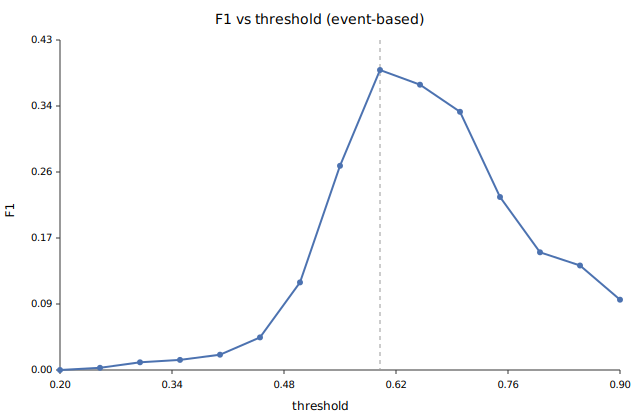
\includegraphics[width=\columnwidth]{figs/f1_vs_threshold.pdf}
\caption{Validation F1 as a function of threshold. The best F1 occurs at 0.6.}
\label{fig:f1_thresh}
\end{figure}

\begin{table}[t]
\caption{Validation performance compared to official baselines and the 2023 winning system.}
\label{tab:results}
\centering
\begin{tabular}{lccc}
\hline
\textbf{Method} & \textbf{Precision} & \textbf{Recall} & \textbf{F1} \\
\hline
Template Matching (baseline) & 2.42 & 18.32 & 4.28 \\
Prototypical Network (baseline) & 36.34 & 24.96 & 29.59 \\
Du et al. (2023 winner) \cite{yanMULTITASKFRAMELEVEL2023} & 76.20 & 75.30 & 75.70 \\
\textbf{Proposed system} & \textbf{45.67} & \textbf{34.06} & \textbf{39.02} \\
\hline
\end{tabular}
\end{table}

Subset‑level precision, recall, and F1 are reported in
Table~\ref{tab:subset_results}. Performance varies by file
(Table~\ref{tab:per_file}): ME and HB recordings tend to be detected reliably,
while PB files with very short events and dense activity show lower recall. This
aligns with the known sensitivity of segment‑level methods to event duration and
annotation density.

\begin{table}[t]
\caption{Per-subset performance for the proposed system.}
\label{tab:subset_results}
\centering
\begin{tabular}{lccc}
\hline
\textbf{Subset} & \textbf{Precision} & \textbf{Recall} & \textbf{F1} \\
\hline
HB & 64.86 & 54.08 & 58.98 \\
ME & 43.12 & 90.38 & 58.39 \\
PB & 36.94 & 25.79 & 30.37 \\
Overall & 45.67 & 34.06 & 39.02 \\
\hline
\end{tabular}
\end{table}

\section{Discussion and Conclusion}
The experiments show that a careful, evaluation‑aware tuning of a lightweight
prototypical pipeline yields clear gains over the official baseline without
external data or heavy backbones. The largest sensitivity comes from post‑processing
threshold choice and minimum‑duration filtering, consistent with the event‑based
metric and the strong class‑imbalance in several files. The gap between subsets
highlights the limitations of segment‑level matching on short, dense events (PB),
where a frame‑level model or stronger temporal modeling would likely help.
Transductive refinement stabilizes file‑to‑file variance, but its impact remains
bounded by the quality of the encoder and the negative sampling strategy.

In conclusion, I implemented a reproducible few‑shot event detection pipeline that
improves the DCASE 2023 prototypical baseline by 9.43 F1 points on the validation
set. The work clarifies which adjustments are most effective under the task rules:
input representation, adaptive segmentation, robust negative sampling, and
post‑processing. Future work should focus on frame‑level scoring, stronger
self‑supervised pretraining within allowed data, and per‑file adaptive thresholds
to further close the gap with state‑of‑the‑art systems.

\bibliographystyle{IEEEtran}
\bibliography{references}

\end{document}
